\documentclass[a4paper,11pt]{article}
\usepackage{amssymb}
\usepackage[polish]{babel}
\usepackage[utf8]{inputenc}
\usepackage[T1]{fontenc}
\usepackage{array}
\usepackage{graphicx}
\usepackage{anysize}
\usepackage{enumerate}
\usepackage{times}
\usepackage{geometry}
\usepackage{amsthm}
\usepackage{pgfplots}
\usepackage{tabularx}
\usepackage{sidecap}
\usepackage{wrapfig}
\usepackage[format=hang,font=small,labelfont=bf]{caption}


\usepackage[intlimits]{amsmath}
\marginsize{3cm}{3cm}{1.5cm}{1.5cm}
\sloppy

\begin{document}
\begin{table}[ht]
\centering
\hspace*{-1cm}
\begin{tabular}{lllllll}
\cline{1-6}
\multicolumn{1}{|c|}{\begin{tabular}[c]{@{}c@{}}EAIiIB\\ Informatyka\end{tabular}}              & \multicolumn{2}{l|}{\begin{tabular}[c]{@{}l@{}}Ewa Stachów\\ Weronika Olcha\end{tabular}}                                                                                                & \multicolumn{1}{c|}{\begin{tabular}[c]{@{}c@{}}Rok\\ II\end{tabular}}          & \multicolumn{1}{c|}{\begin{tabular}[c]{@{}c@{}}Grupa\\ 3\end{tabular}}            & \multicolumn{1}{c|}{\begin{tabular}[c]{@{}c@{}}Zespół\\ 6\end{tabular}}      &  \\ \cline{1-6}
\multicolumn{1}{|c|}{\begin{tabular}[c]{@{}c@{}}Pracownia\\ FIZYCZNA\\ WFiIS AGH\end{tabular}} & \multicolumn{4}{l|}{\begin{tabular}[c]{@{}l@{}}Temat:\\ \textbf{\textit{Mostek Wheastone'a}} \end{tabular}}                                                                                                                                                                                                                                            & \multicolumn{1}{c|}{\begin{tabular}[c]{@{}c@{}}Nr ćwiczenia:\\ 32\end{tabular}} &  \\ \cline{1-6}
\multicolumn{1}{|l|}{\begin{tabular}[c]{@{}c@{}}Data wykonania:\\ 21.10.2016\end{tabular}}      & \multicolumn{1}{c|}{\begin{tabular}[c]{@{}c@{}}Data oddania:\\ 26.10.2016\end{tabular}} & \multicolumn{1}{l|}{\begin{tabular}[c]{@{}l@{}}Zwrot do poprawki:\\ \phantom{data poprawki}\end{tabular}} & \multicolumn{1}{l|}{\begin{tabular}[c]{@{}l@{}}Data oddania:\\  \phantom{data oddania}\end{tabular}} & \multicolumn{1}{l|}{\begin{tabular}[c]{@{}l@{}}Data zaliczenia:\\  \phantom{data zaliczenia}\end{tabular}} & \multicolumn{1}{l|}{\begin{tabular}[c]{@{}l@{}}OCENA:\\ \phantom{ocena}\end{tabular}}       &  \\ \cline{1-6}
                                                                                                
\end{tabular}
\end{table}

\begin{center}
\begin{LARGE}
\textbf{Ćwiczenie nr 32: Mostek Wheastone'a}
\end{LARGE}
\end{center}

\section{Cel ćwiczenia}
Celem ćwiczenia było zapoznanie z zasadą działania mostka Wheatstone’a w oparciu o prądowe i napięciowe prawo Kirchoffa służące do opisu złożonych obwodów elektrycznych oraz metody pomiaru nieznanych oporów oraz ich połączeń szeregowych i równoległych zgodnie z prawem Ohma.

\section{Wstęp teoretyczny}
\begin{wrapfigure}{l}{0.4\textwidth}
\vspace*{-0.5cm}
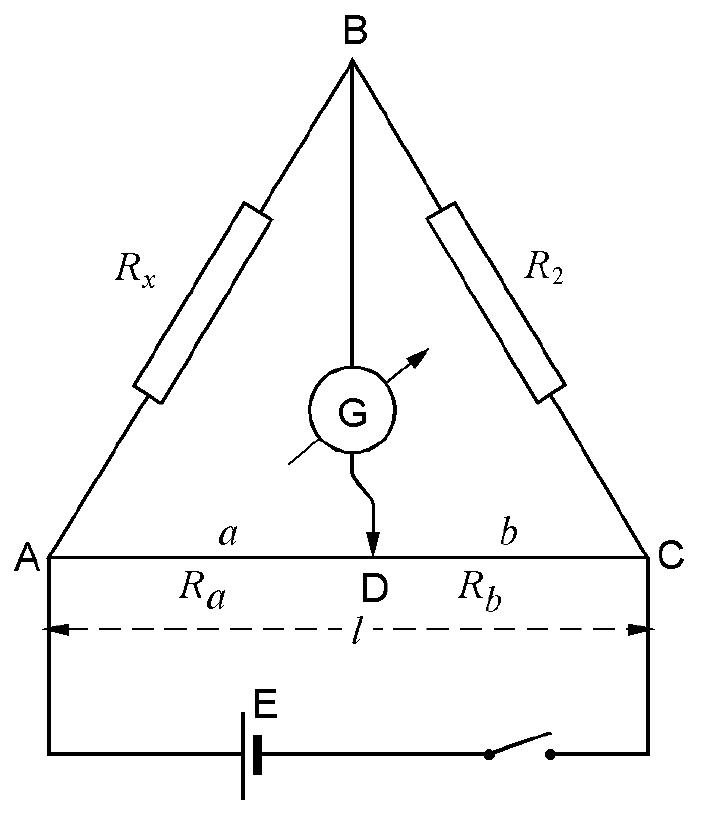
\includegraphics[width=0.4\textwidth]{./schemat}
\end{wrapfigure}
Mostek Wheatstone’a jest jednym z klasycznych sposobów dokładnego pomiaru nieznanego oporu elektrycznego. Załóżmy, że mamy nieznany opór $R_x$, znane opory $R_a$, $R_b$ oraz regulowaną opornicę dekadową o oporze $R_2$. Zestawiamy następujący obwód: do szeregowego połączenia oporów $R_x$, $R_2$ przyłączamy równolegle połączenie szeregowe $R_a$, $R_b$. Węzły pomiędzy wspomnianymi parami oporów łączymy galwanometrem. Po przyłożeniu do układu różnicy potencjałów możemy regulować $R_2$ tak, aby galwanometr wskazywał 0, czyli brak różnicy potencjałów, a co za tym idzie i brak przepływu prądu między odpowiednimi węzłami. Wtedy z praw Ohma i Kirchhoffa możemy wyprowadzić następujące wzory: 
$$I_a\cdot R_a=I_x\cdot R_x$$
$$I_b\cdot R_b=I_d\cdot R_2$$
Z powyższych równań wynika równość spadków napięć na odpowiednich oporach oraz równość odpowiednich natężeń prądów, czyli:
$$I_a=I_b$$
$$I_x=I_d$$
Stąd można wyprowadzić wyrażenie na $R_x$:
$$R_x=R_a\frac{I_a}{I_x}=R_a\frac{I_b}{I_d}=R_2\frac{R_a}{R_b}$$
Ponieważ $R_a$ i $R_b$ są oporami odcinków tego samego jednorodnego drutu, ich wielkości są proporcjonalne do długości:
$$\frac{R_a}{R_b}=\dfrac{a}{b}=\dfrac{a}{l-a}$$
Ostatecznie otrzymujemy, że:
$$R_x=R_2\dfrac{a}{l-a}$$
Dokładność pomiaru mostkiem Wheatstone’a z drutem oporowym zależy przede wszystkim od błędu wyznaczenia odległości $a$. Aby pomiar był najdokładniejszy należy tak dobrać opór $R_2$, aby stan równowagi mostka można było uzyskać w przybliżeniu w połowie długości drutu oporowego.

\section{Układ pomiarowy}
Układ mostka Wheatstone’a pokazany został na rysunku w punkcie nr 2 \textit{Wstęp teoretyczny}. W~skład obwodu wchodzą:
\begin{itemize}
\item Listwa z drutem oporowym, zaopatrzona w podziałkę milimetrową i kontakt ślizgowy umożliwiający zmiany długości odcinków $a$ i $b$.
\item  Opornica dekadowa
\item  Zestaw oporników oznaczony symbolem $R_x$, umieszczony na płytce z pleksiglasu.
\item Mikroamperomierz $G$ jako wskaźnik zerowania mostka. Jego czułość można regulować.
\item Zasilacz.
\end{itemize}

\section{Przebieg doświadczenia}
Przy przeprowadzaniu eksperymentu skorzystałyśmy z układu pomiarowego, którego schemat przedstawia poniższy rysunek. Pomiędzy punktami $A$ i $C$ znajduje się listwa z  drutem oporowym o znanej długości. $R_2$ jest opornikiem wzorcowym o regulowanej wartości oporu, a $R_x$ nieznanym oporem, którego wartość chcemy wyznaczyć. Zrównoważenie mostka polega na takim ustawieniu punktu $D$, aby dla zadanej wartości $R_2$ przez galwanometr nie płynął prąd.

\section{Wyniki pomiarów}


\begin{table}[!ht]
\setlength{\extrarowheight}{5pt}
\centering
\begin{tabularx}{\textwidth}{XXXXXXXXXXX}

\multicolumn{11}{c}{\textbf{Opornik $R_1$}}\\        
\hline
$R_1[\Omega]$  & 25 & 20 & 30 & 15 & 13 & 10 & 8 & 5 & 18 & 23 \\
\hline
$a[mm]$  & 354 & 427 & 331 & 472 & 512 & 599 & 612 & 682 & 427 & 378  \\
\hline
$R_{x_1}[\Omega]$ & 13,70 &	14,90 &	14,84 &	13,41 &	13,64 &	14,94 &	12,62 &	10,72 &	13,41 &	13,98
\\    
\hline   
\end{tabularx}
\begin{tabularx}{\textwidth}{XX}
\centering
Wartość średnia oporu: $\overline{R}_{x_1}= 13,62~\Omega$ & Niepewność: $u(R_{x_1})=0,40 ~\Omega $\\

\end{tabularx}
\end{table}

\begin{table}[!ht]
\setlength{\extrarowheight}{5pt}
\centering
\begin{tabularx}{\textwidth}{XXXXXXXXXXX}

\multicolumn{11}{c}{\textbf{Opornik $R_2$}}\\        
\hline
$R_2[\Omega]$  &20	&30	&10	&35	&25	&15	&18	&12	&22	&28   \\
\hline
$a[mm]$  & 504 & 407 & 675 & 358 & 438 & 556 & 515 & 619	& 477 & 411 \\
\hline
$R_{x_2}[\Omega]$ &20,32 &20,59 &20,77 &19,52 &19,48 &18,78	&19,11	&19,50	&20,07	&19,54
\\    
\hline   
\end{tabularx}
\begin{tabularx}{\textwidth}{XX}
\centering
Wartość średnia oporu: $\overline{R}_{x_2}\approx 19,77~\Omega $ & Niepewność: $u(R_{x_2})\approx 0,20 ~\Omega $\\

\end{tabularx}
\end{table}


         
\begin{table}[!ht]
\setlength{\extrarowheight}{5pt}
\centering
\begin{tabularx}{\textwidth}{XXXXXXXXXXX}

\multicolumn{11}{c}{\textbf{Połączenie szeregowe ($R_1$ z $R_2$)}}\\        
\hline
$R_{12}[\Omega]$  & 20	&30	&35	&40	&50	&45	&25	&28	&32	&38 \\
\hline
$a[mm]$  & 640	&531 &500 &461 &414 &436 &575 &545 &526	&479 \\
\hline
$R_{z_s}[\Omega]$ & 35,56 & 33,97 & 35,00 & 34,21 & 35,32 & 34,79 & 33,82 & 33,54 & 35,51 & 34,94
\\    
\hline   
\end{tabularx}
\begin{tabularx}{\textwidth}{XX}
\centering
Wartość średnia oporu: $\overline{R}_{z_s}\approx 34,67~\Omega$ & Niepewność: $u(R_{z_s})\approx 0,23~\Omega$ \\ \hline
\centering
Opór obliczony: $R_{obl} \approx 33,38~\Omega$ & Niepewność: $u(R_{obl})\approx 0,45~\Omega$\\
\end{tabularx}
\end{table}

\begin{table}[!ht]
\setlength{\extrarowheight}{5pt}
\centering
\begin{tabularx}{\textwidth}{XXXXXXXXXXX}

\multicolumn{11}{c}{\textbf{Połączenie równoległe ($R_1$ z $R_2$)}}\\        
\hline
$R_{12}[\Omega]$  & 3 &4 &5 &6 &7 &8 &9 &10 &11 &13\\
\hline
$a[mm]$  & 662 & 592 & 560 & 526 & 496 & 467 & 434 & 461 & 427 & 371
  \\
\hline
$R_{z_r}[\Omega]$ & 5,88 &5,80&6,36 &6,66 &6,89	&7,01 &6,90	&8,55 &8,20	&7,67
\\    
\hline   
\end{tabularx}
\begin{tabularx}{\textwidth}{XX}
\centering
Wartość średnia oporu: $\overline{R}_{z_r}\approx6,99~\Omega $ & Niepewność: $u(R_{z_r})\approx 0,29~\Omega$ \\ \hline
\centering
Opór obliczony: $R_{obl} \approx 8,06~\Omega$ & Niepewność: $u(R_{obl})\approx 0,10 ~\Omega$\\
\end{tabularx}
\end{table}


\section{Opracowanie wyników pomiarów}
Aby obliczyć opór $R_x$ korzystamy z poniższego wzoru:
$$
R_x = R_2 \frac{a}{l-a},
$$
gdzie $R_2$ to znana opór wzorcowy, $a$ to zmierzona długość, a $l=1000mm$ to długość  listwy z~drutem oporowym.
Niepewność typu A wartości $R_x$ wyznaczamy z następującego wzoru:
$$
u(R_x) = \sqrt{\frac{\sum \left( R_i - \overline{R}_x \right)^2 }{n(n-1)}}
$$
Po podstawieniu odpowiednich wartości otrzymujemy:
$$
u(R_1) = \sqrt{\frac{(13,70-13,62)^2 + \cdots (13,98-13,62)^2  }{10(10-1)}}\approx 0,40 ~\Omega
$$

$$
u(R_2) = \sqrt{\frac{(20,32-19,77)^2 + \cdots (19,54-19,77)^2  }{10(10-1)}} \approx 0,20 ~\Omega
$$

$$
u(R_{z_s}) = \sqrt{\frac{(35,56-34,67)^2 + \cdots (34,94-34,67)^2  }{10(10-1)}} \approx 0,23 ~\Omega
$$

$$
u(R_{z_r}) = \sqrt{\frac{(5,88-6,99)^2 + \cdots (7,67-6,99)^2  }{10(10-1)}} \approx 0,29 ~\Omega
$$
\subsection{Połączenie szeregowe}
Wartość oporu przy połączeniu szeregowym można też obliczyć na podstawie wzoru na opór zastępczy oraz wyznaczonych wartości $R_{x_1}$ i  $R_{x_2}$

$$
R_{obl} = R_{x_1} + R_{x_2} \approx 33,38~\Omega
$$
Niepewność dla wartości wyliczanych ze wzorów na opór zastępczy w obwodzie z połączeniem szeregowym wyznaczamy z prawa przenoszenia niepewności i opisujemy wzorem:
\begin{center}
\begin{align*}
u(R_{obl}) &= \sqrt{\left( \frac{\delta R_{z_{s}} }{\delta R_{x_1}}  \right)^2 u(R_{x_1})^2  +\left( \frac{\delta R_{z_{s}} }{\delta R_{x_2}}  \right)^2  u(R_{x_2})^2  } \\
& = \sqrt{u(R_{x_1})^2 + u(R_{x_2})^2} \\
&\approx  0,45 ~\Omega
\end{align*}
\end{center}


\subsection{Połączenie równoległe}
Wartość oporu przy połączeniu równoległym można też obliczyć na podstawie wzoru na opór zastępczy oraz wyznaczonych wartości $R_{x_1}$ i  $R_{x_2}$

$$ 
R_{z_r} = \frac{ R_{x_1} R_{x_2}}{ R_{x_1} + R_{x_2}} \approx 8,06~\Omega
$$
\begin{center}
\begin{align*}
u(R_{obl}) &= \sqrt{\left( \frac{\delta R_{z_r} }{\delta R_{x_1}}  \right)^2 u(R_{x_1})^2  +\left( \frac{\delta R_{z_r} }{\delta R_{x_2}}  \right)^2  u(R_{x_2})^2  }\\ 
& =  \sqrt{\left(  \frac{R_{x_1}}{R_{x_1} + R_{x_2}}\right)^4  u(R_{x_1})^2 + \left(\frac{R_{x_2}}{R_{x_1} + R_{x_2}}\right)^4  u(R_{x_2})^2}\\ 
&\approx  0,10~\Omega
\end{align*}
\end{center}


\subsection{Porównanie wartości z pomiarów i wyznaczonych ze wzorów}
\begin{tabularx}{\textwidth}{XXX}
\hline
 & \textbf{Opory zmierzone}  & \textbf{Opory ze wzoru} \\ 
\hline \textbf{Połączenie szeregowe} & $34,67(23) ~\Omega$ & $33,38(45) ~\Omega$ \\ 
\hline \textbf{Połączenie równoległe} & $6,99(29)~\Omega$& $8,06(10) ~\Omega$\\ 
\hline 
\end{tabularx} 
\section{Wnioski}
\begin{itemize} 
\item Opory wyznaczone w ćwiczeniu mają zbliżone wartości do obliczonych ze wzorów, jednak nie mieszczą się w granicach niepewności pomiarowych (nawet w granicach niepewności rozszerzonej dla współczynnika rozszerzenia $k=2$.).
\item Błędy mogą wynikać ze złego odczytania wartości z amperomierza, bądź złego odczytania długości drutu, lub niedokładności urządzeń pomiarowych.
 
\end{itemize}



\end{document}